\chapter{Resultados}
Nesse capítulo é apresentado como os testes foram organizados, as limitações do software, os resultados encontrados e futuras melhorias.

\section{Limitações}
Foi possível identificar possíveis situações em que o software não foi capaz de dar uma resposta, estes sendo:

\textbf{Não é possível entregar a tempo}: Levando em consideração o horário de saída e o horário limite para realizar todas as entregas, é possível que um percurso entre os endereços tem seu tempo de trajeto mais demorado que o tempo disponível para a realização de todas as entregas, com isso seria impossível entregar, mesmo com mais entregadores, com isso, o software não consegue definir uma rota por considerar a velocidade média das vias por onde ele passará.

\textbf{Limite de Entregadores:} Para pedir a definição de uma rota é preciso indicar quantos entregadores estão disponível para realizar as entregas, em algumas situações é possível que mesmo dividindo para todos os entregadores, mais entregadores seriam precisos para chegar a tempo em todos os endereços, com isso, o software não consegue definir uma rota.

\textbf{Tempo limite de entrega excedido:} Se a rota não tiver nenhum percurso muito demorado e também for possível determinar a divisão da rota principal entre o numero de entregadores, podemos encontrar outro problema, sempre que um entregador chega a um destino, é possível sofre atrasos na descarga, um maior tempo de espera ou até o transito piorando por causa de um acidente em uma via principal, por exemplo, isso muda o tempo dos próximos percursos, podendo elevar muito o tempo do trajeto.

É possível encontrar a situação que seria preciso mais entregadores para finalizar a entrega, que não é mais possível por que o entregador já está em transito, também pode encontrar um percurso completamente parado,  com isso, o software não consegue definir uma rota para finalizar as entregas.


\section{Comparativo}
Com diferentes tipos de mutação, foi preciso escolher apenas um para rodar todos os roteiros, para comparação foi utilizado os diferentes tipos de mutação e apenas um cruzamento, de forma, a identificar uma melhor combinação para ser utilizada no software, 10 vezes para cada combinação utilizando a média do valor de aptidão para evitar o efeito probabilístico do GA. Utilizando o projeto Route.DataGeneration, todas os dados das possibilidades foram armazenados em um arquivo csv e organizado na tabela a baixo. 

\begin{center}
	\makebox[\linewidth]{
		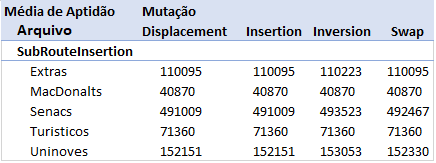
\includegraphics[keepaspectratio=true,scale=1.4]{ibagens/MutacaoComparacao.png}}
	\captionof{figure}{Comparação das Mutações}
	\label{fig:MutacaoComparacao}
\end{center}

Como mostrado na tabela \ref{fig:MutacaoComparacao}, o Inversion e o Swap não conseguiram a menor média em todos os arquivos, parecendo não recomendado o uso para a criação das rotas. O Displacement e o Insertion encontraram a mesma média de aptião para todas os arquivos, mostrando serem as melhores escolhas para a busca de rotas.

\pagebreak
\section{Roteiros dos Testes}
Os roteiros foram escolhidos de forma arbitraria com endereços dentro ou próximos da cidade de São Paulo. As listas de endereços e as rotas encontrada podem ser vista a baixo:

\subsection{Roteiro 1}
\begin{center}
	\makebox[\linewidth]{
		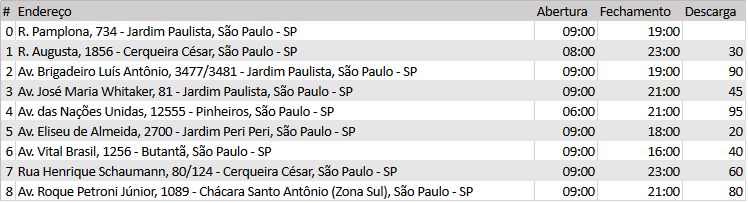
\includegraphics[keepaspectratio=true,scale=0.9]{../../Analise/Roteiro1/Tabela.png}}
	\captionof{figure}{Roteiro de um entregador}
	\label{fig:Roteiro1}
\end{center}
\begin{center}
	\makebox[\linewidth]{
		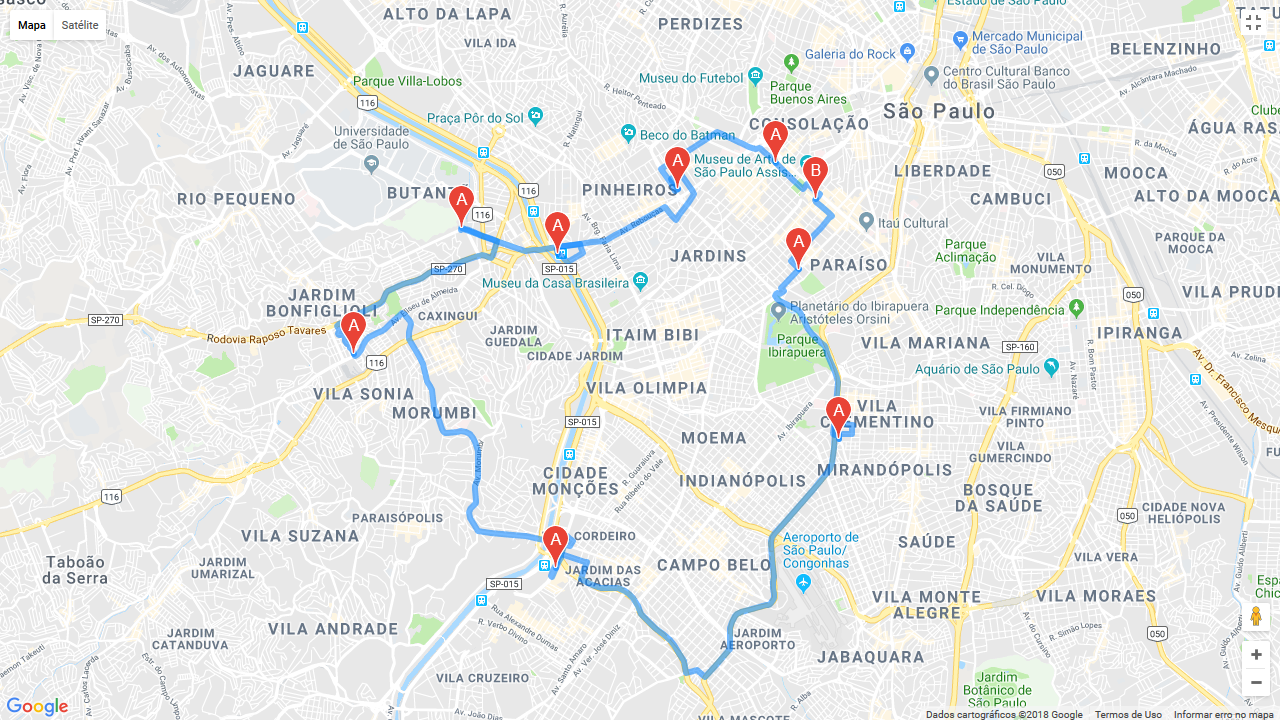
\includegraphics[keepaspectratio=true,scale=0.5]{../../Analise/Roteiro1/Mapa1.png}}
	\captionof{figure}{Mapa de um entregador}
	\label{fig:Roteiro1-Mapa1}
\end{center}

\subsubsection{500 Gerações e 50 População}
\begin{center}
	\makebox[\linewidth]{
		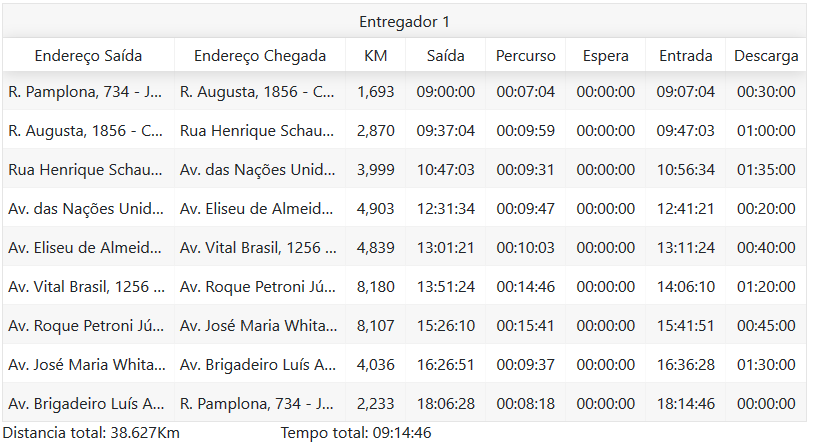
\includegraphics[keepaspectratio=true,scale=0.8]{../../Analise/Roteiro1/G500P50/DisplacementMutation.png}}
	\captionof{figure}{Mutação DisplacementMutation}
	\label{fig:Roteiro1-G500P50-DisplacementMutation}
\end{center}
\begin{center}
	\makebox[\linewidth]{
		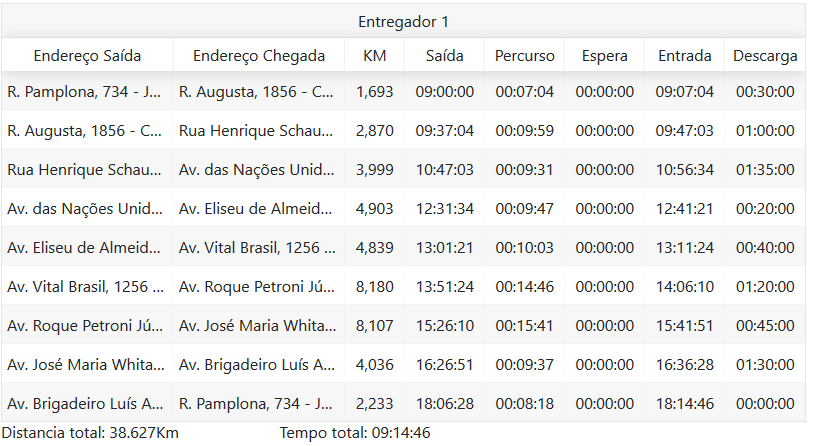
\includegraphics[keepaspectratio=true,scale=0.8]{../../Analise/Roteiro1/G500P50/InsertionMutation.png}}
	\captionof{figure}{Mutação InsertionMutation}
	\label{fig:Roteiro1-G500P50-InsertionMutation}
\end{center}
\begin{center}
	\makebox[\linewidth]{
		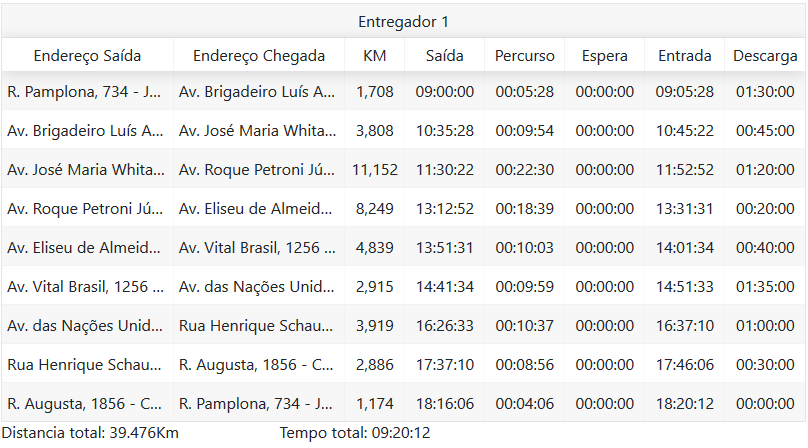
\includegraphics[keepaspectratio=true,scale=0.8]{../../Analise/Roteiro1/G500P50/InversionMutation.png}}
	\captionof{figure}{Mutação InversionMutation}
	\label{fig:Roteiro1-G500P50-InversionMutation}
\end{center}
\begin{center}
	\makebox[\linewidth]{
		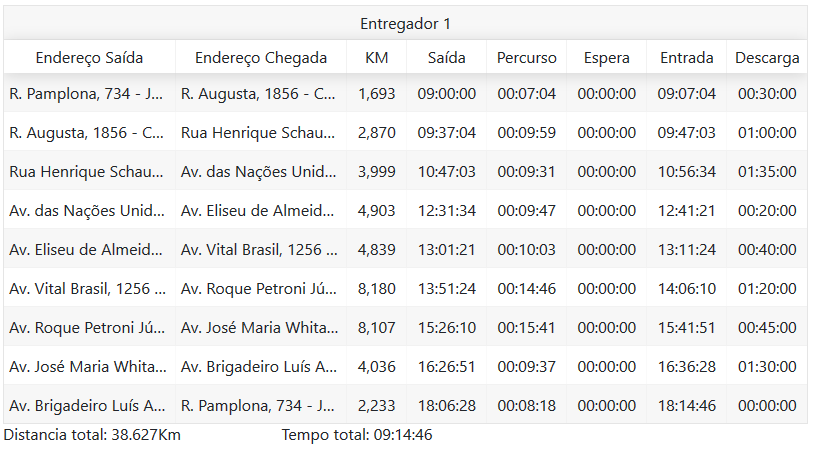
\includegraphics[keepaspectratio=true,scale=0.8]{../../Analise/Roteiro1/G500P50/SwapMutation.png}}
	\captionof{figure}{Mutação SwapMutation}
	\label{fig:Roteiro1-G500P50-SwapMutation}
\end{center}

\subsubsection{1000 Gerações e 100 População}
\begin{center}
	\makebox[\linewidth]{
		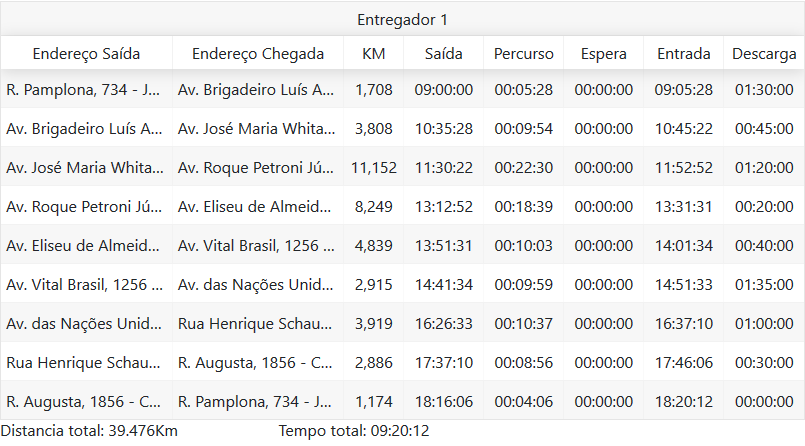
\includegraphics[keepaspectratio=true,scale=0.8]{../../Analise/Roteiro1/G1000P100/DisplacementMutation.png}}
	\captionof{figure}{Mutação DisplacementMutation}
	\label{fig:Roteiro1-G1000P100-DisplacementMutation}
\end{center}
\begin{center}
	\makebox[\linewidth]{
		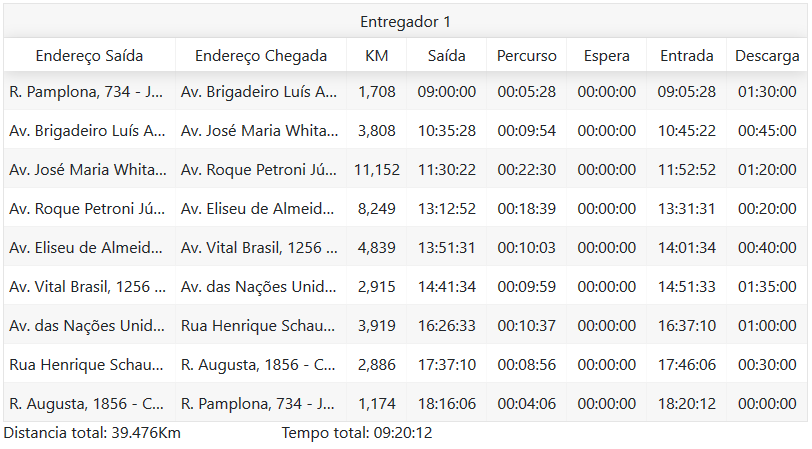
\includegraphics[keepaspectratio=true,scale=0.8]{../../Analise/Roteiro1/G1000P100/InsertionMutation.png}}
	\captionof{figure}{Mutação InsertionMutation}
	\label{fig:Roteiro1-G1000P100-InsertionMutation}
\end{center}
\begin{center}
	\makebox[\linewidth]{
		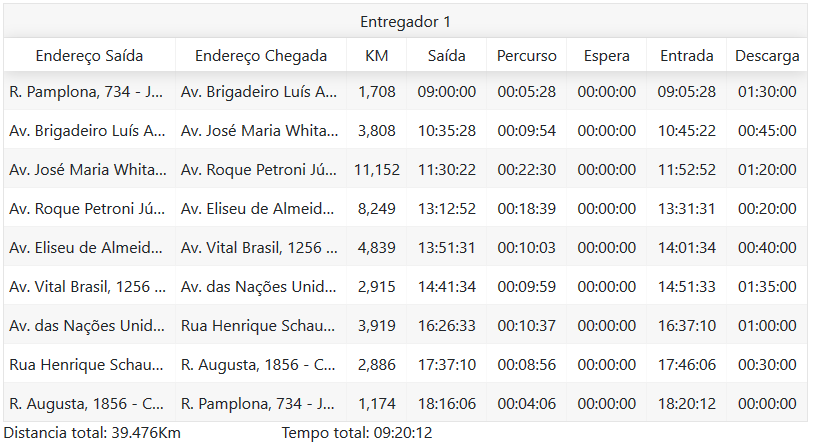
\includegraphics[keepaspectratio=true,scale=0.8]{../../Analise/Roteiro1/G1000P100/InversionMutation.png}}
	\captionof{figure}{Mutação InversionMutation}
	\label{fig:Roteiro1-G1000P100-InversionMutation}
\end{center}
\begin{center}
	\makebox[\linewidth]{
		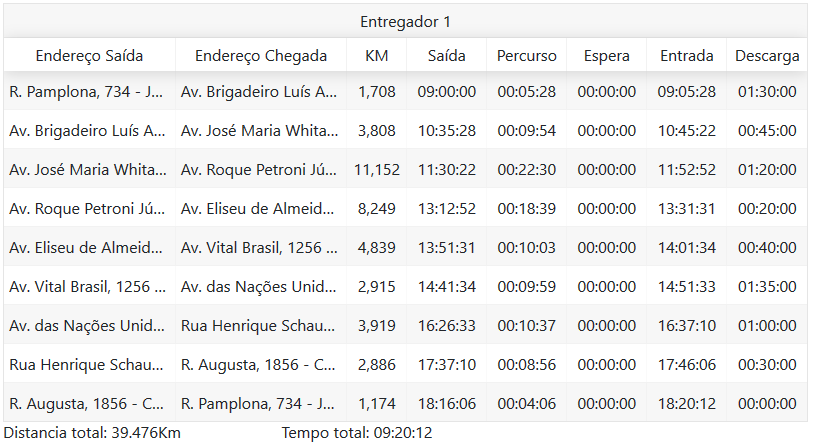
\includegraphics[keepaspectratio=true,scale=0.8]{../../Analise/Roteiro1/G1000P100/SwapMutation.png}}
	\captionof{figure}{Mutação SwapMutation}
	\label{fig:Roteiro1-G1000P100-SwapMutation}
\end{center}


\subsection{Roteiro 2}
\begin{center}
	\makebox[\linewidth]{
		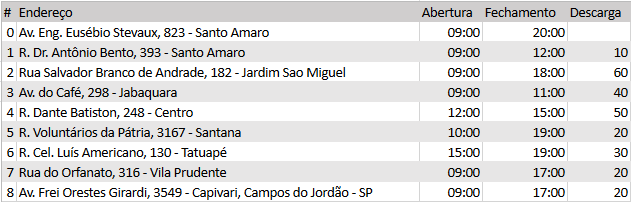
\includegraphics[keepaspectratio=true,scale=0.9]{../../Analise/Roteiro2/Tabela.png}}
	\captionof{figure}{Roteiro de dois entregadores}
	\label{fig:Roteiro2}
\end{center}
\begin{center}
	\makebox[\linewidth]{
		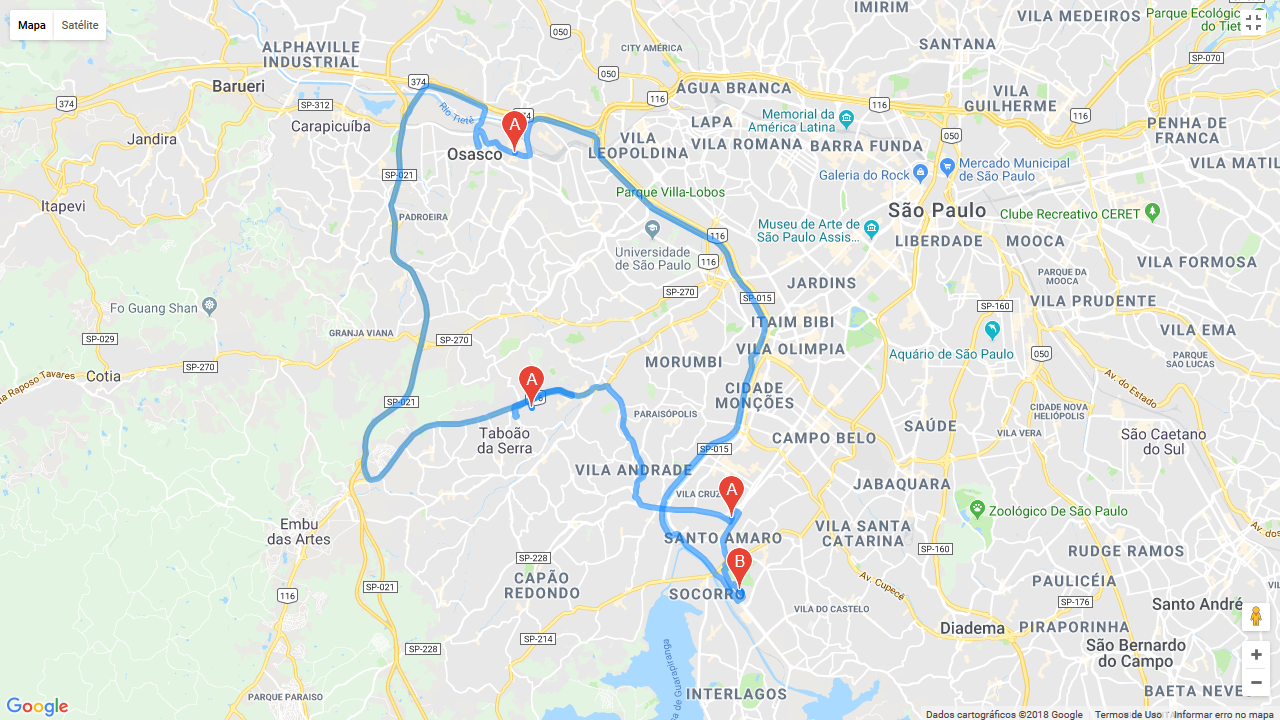
\includegraphics[keepaspectratio=true,scale=0.5]{../../Analise/Roteiro2/Mapa1.png}}
	\captionof{figure}{Mapa de um de dois entregadores}
	\label{fig:Roteiro2-Mapa1}
\end{center}
\begin{center}
	\makebox[\linewidth]{
		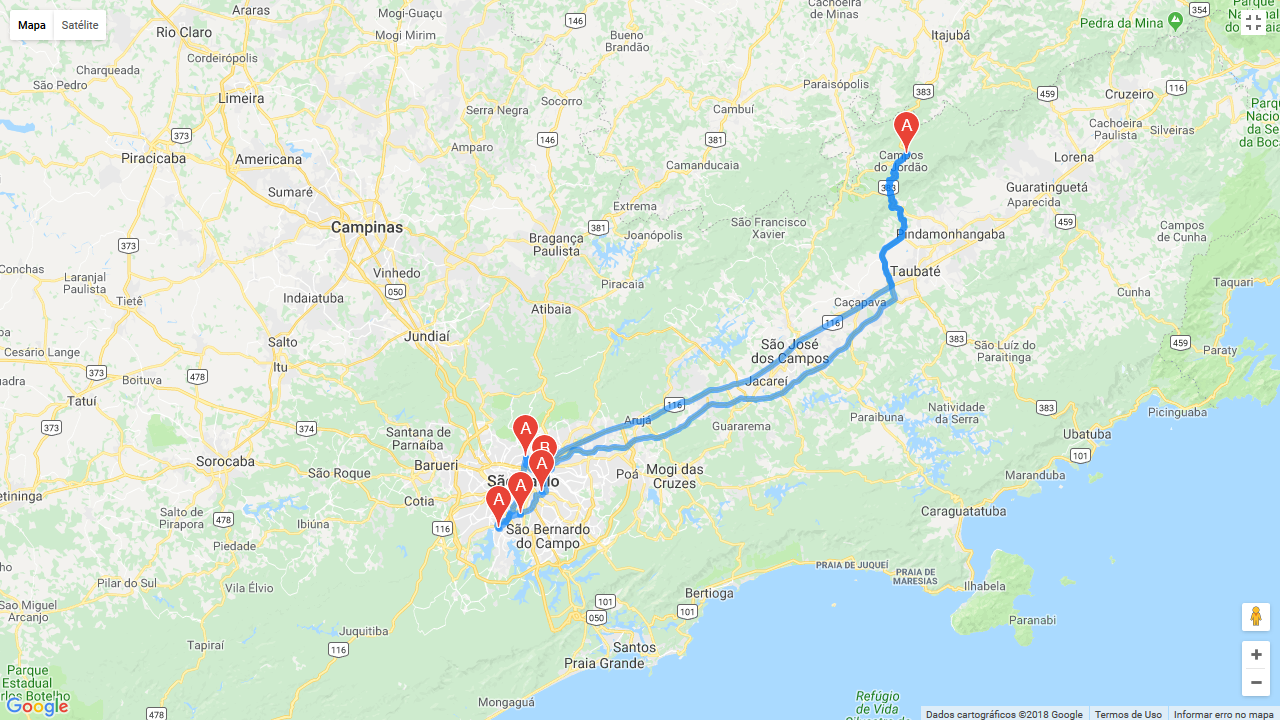
\includegraphics[keepaspectratio=true,scale=0.5]{../../Analise/Roteiro2/Mapa2.png}}
	\captionof{figure}{Mapa de um de dois entregadores}
	\label{fig:Roteiro2-Mapa2}
\end{center}


\subsubsection{500 Gerações e 50 População}
\begin{center}
	\makebox[\linewidth]{
		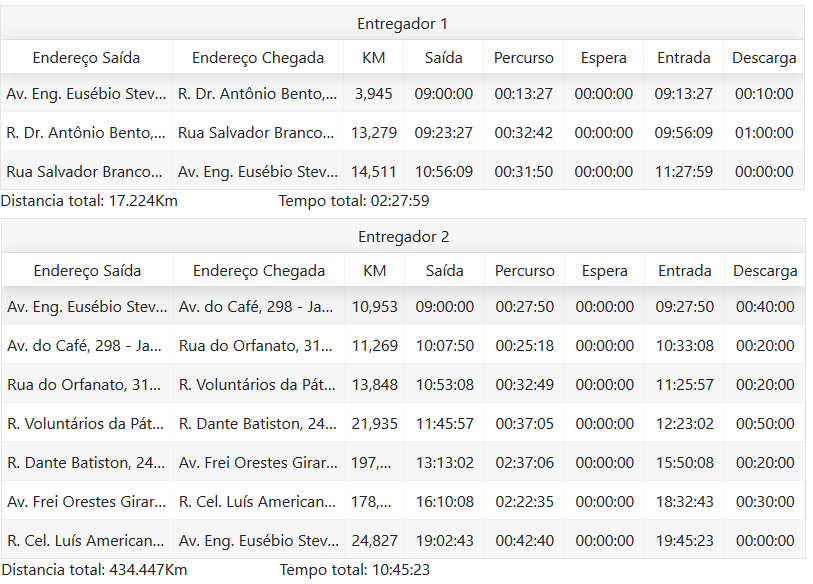
\includegraphics[keepaspectratio=true,scale=0.8]{../../Analise/Roteiro2/G500P50/DisplacementMutation.png}}
	\captionof{figure}{Mutação DisplacementMutation}
	\label{fig:Roteiro2-G500P50-DisplacementMutation}
\end{center}
\begin{center}
	\makebox[\linewidth]{
		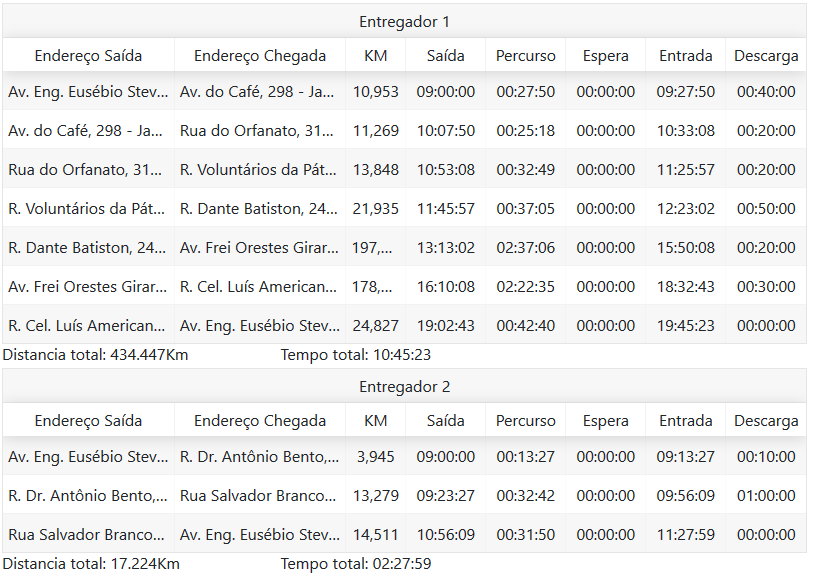
\includegraphics[keepaspectratio=true,scale=0.8]{../../Analise/Roteiro2/G500P50/InsertionMutation.png}}
	\captionof{figure}{Mutação InsertionMutation}
	\label{fig:Roteiro2-G500P50-InsertionMutation}
\end{center}
\begin{center}
	\makebox[\linewidth]{
		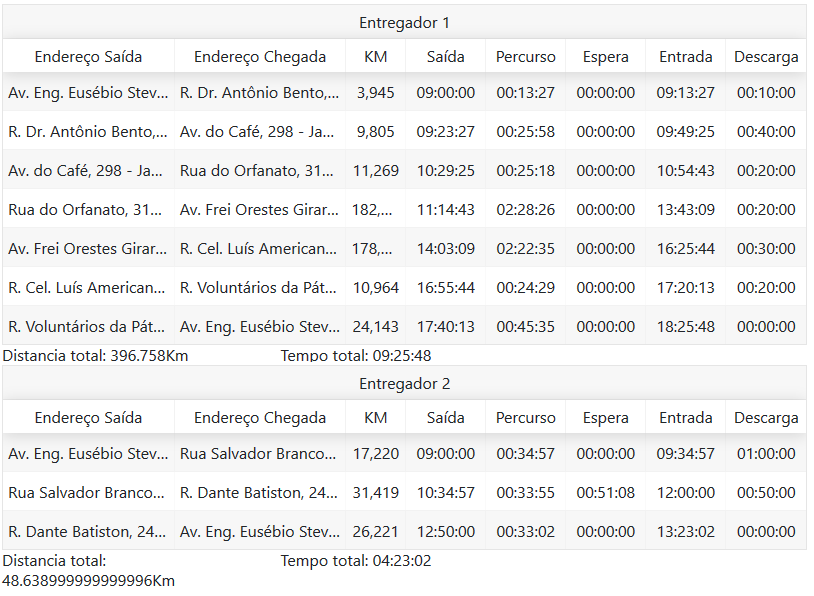
\includegraphics[keepaspectratio=true,scale=0.8]{../../Analise/Roteiro2/G500P50/InversionMutation.png}}
	\captionof{figure}{Mutação InversionMutation}
	\label{fig:Roteiro2-G500P50-InversionMutation}
\end{center}
\begin{center}
	\makebox[\linewidth]{
		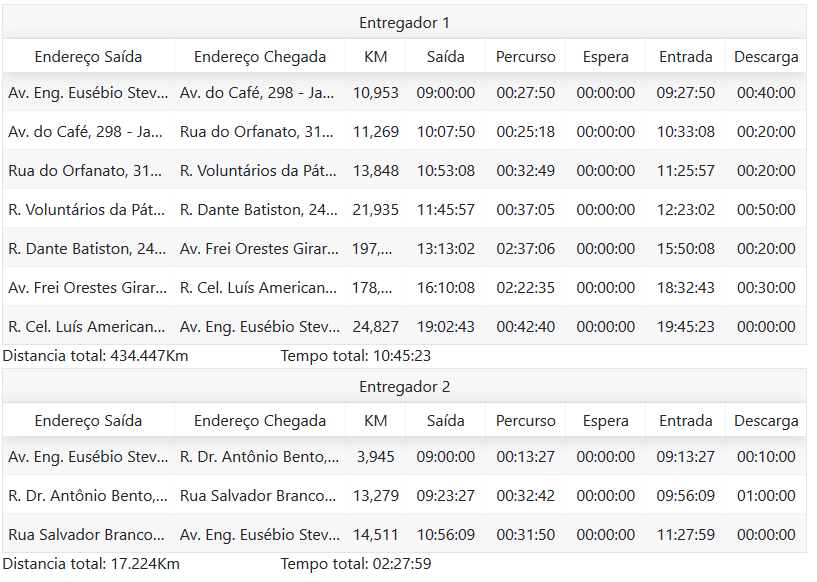
\includegraphics[keepaspectratio=true,scale=0.8]{../../Analise/Roteiro2/G500P50/SwapMutation.png}}
	\captionof{figure}{Mutação SwapMutation}
	\label{fig:Roteiro2-G500P50-SwapMutation}
\end{center}

\subsubsection{1000 Gerações e 100 População}
\begin{center}
	\makebox[\linewidth]{
		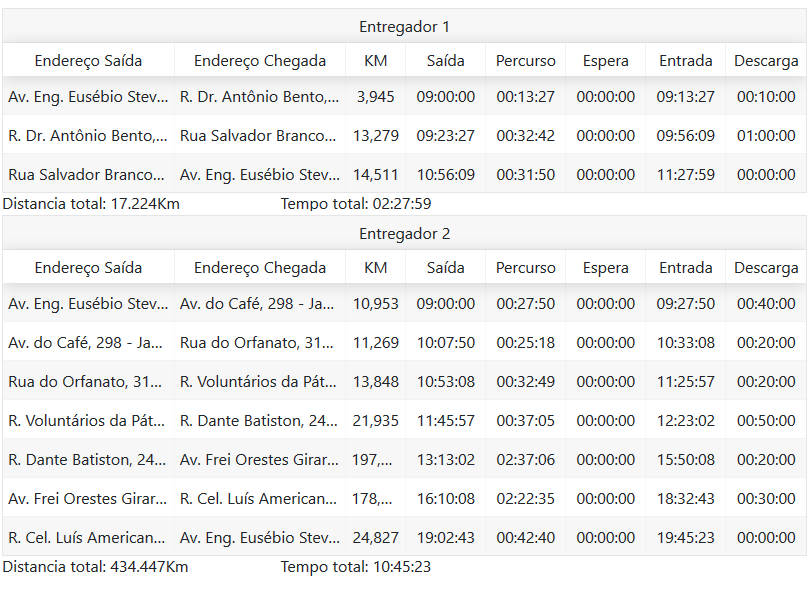
\includegraphics[keepaspectratio=true,scale=0.8]{../../Analise/Roteiro2/G1000P100/DisplacementMutation.png}}
	\captionof{figure}{Mutação DisplacementMutation}
	\label{fig:Roteiro2-G1000P100-DisplacementMutation}
\end{center}
\begin{center}
	\makebox[\linewidth]{
		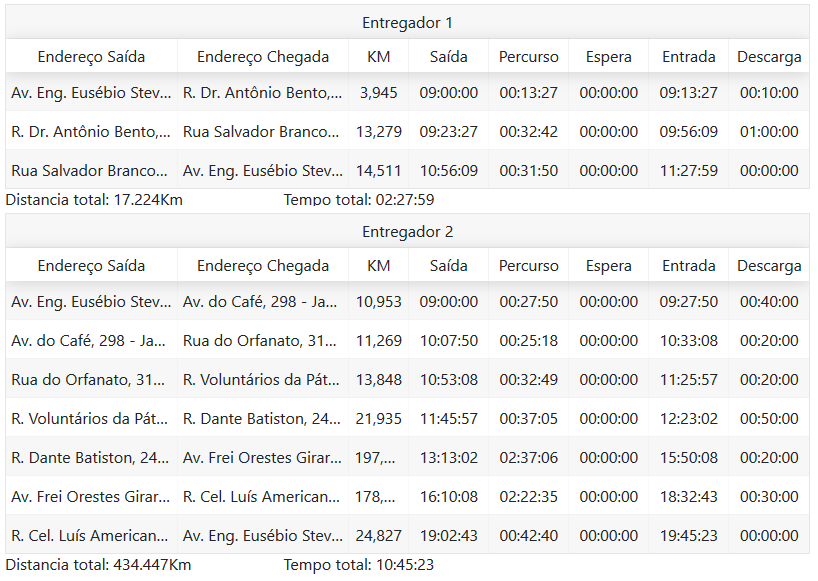
\includegraphics[keepaspectratio=true,scale=0.8]{../../Analise/Roteiro2/G1000P100/InsertionMutation.png}}
	\captionof{figure}{Mutação InsertionMutation}
	\label{fig:Roteiro2-G1000P100-InsertionMutation}
\end{center}
\begin{center}
	\makebox[\linewidth]{
		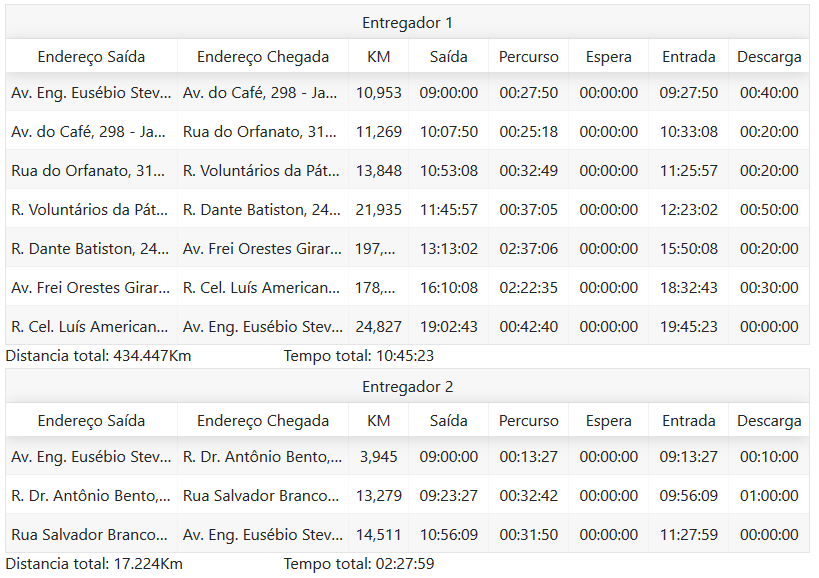
\includegraphics[keepaspectratio=true,scale=0.8]{../../Analise/Roteiro2/G1000P100/InversionMutation.png}}
	\captionof{figure}{Mutação InversionMutation}
	\label{fig:Roteiro2-G1000P100-InversionMutation}
\end{center}
\begin{center}
	\makebox[\linewidth]{
		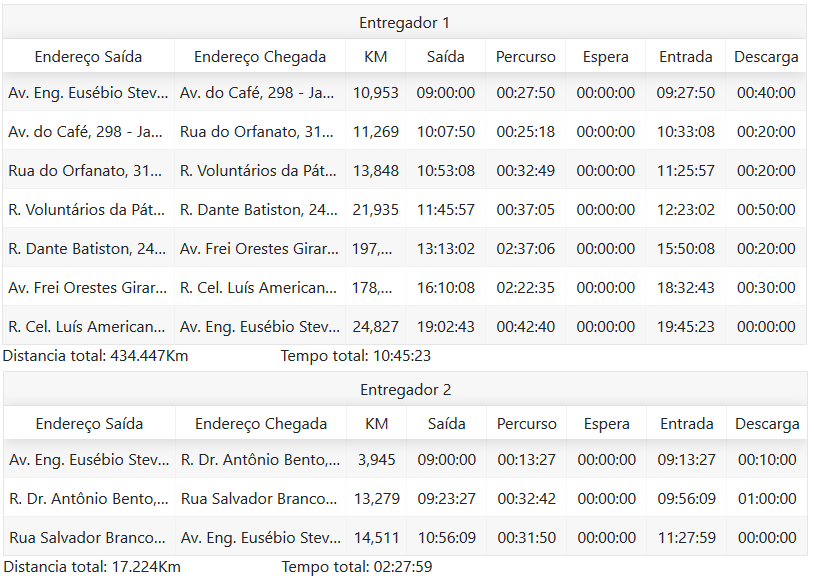
\includegraphics[keepaspectratio=true,scale=0.8]{../../Analise/Roteiro2/G1000P100/SwapMutation.png}}
	\captionof{figure}{Mutação SwapMutation}
	\label{fig:Roteiro2-G1000P100-SwapMutation}
\end{center}


\subsection{Roteiro 3}
\begin{center}
	\makebox[\linewidth]{
		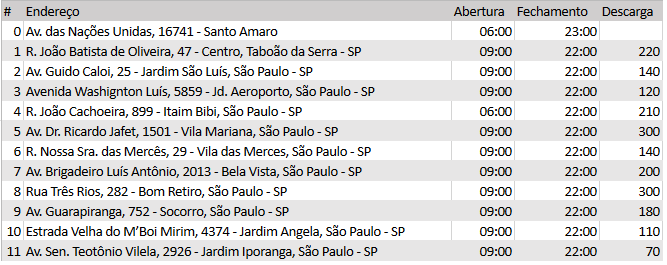
\includegraphics[keepaspectratio=true,scale=0.9]{../../Analise/Roteiro3/Tabela.png}}
	\captionof{figure}{Roteiro de tres entregadores}
	\label{fig:Roteiro3}
\end{center}
\begin{center}
	\makebox[\linewidth]{
		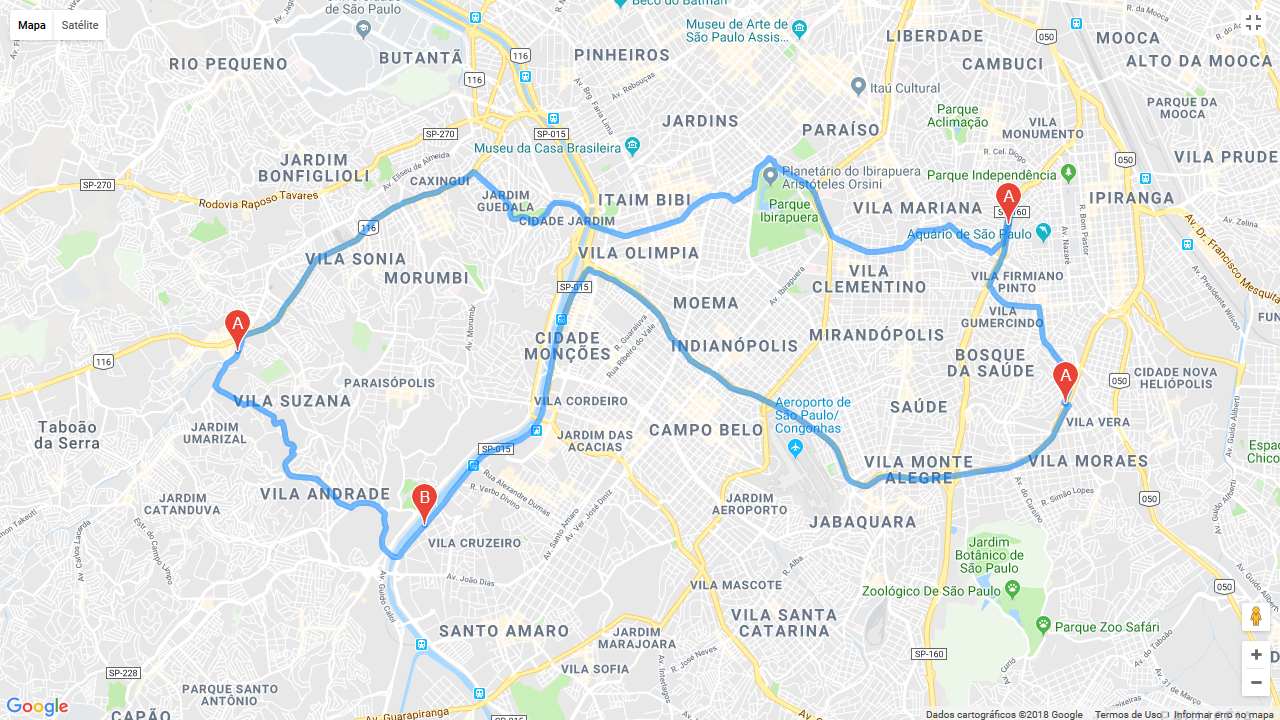
\includegraphics[keepaspectratio=true,scale=0.5]{../../Analise/Roteiro3/Mapa1.png}}
	\captionof{figure}{Mapa de um de tres entregadores}
	\label{fig:Roteiro3-Mapa1}
\end{center}
\begin{center}
	\makebox[\linewidth]{
		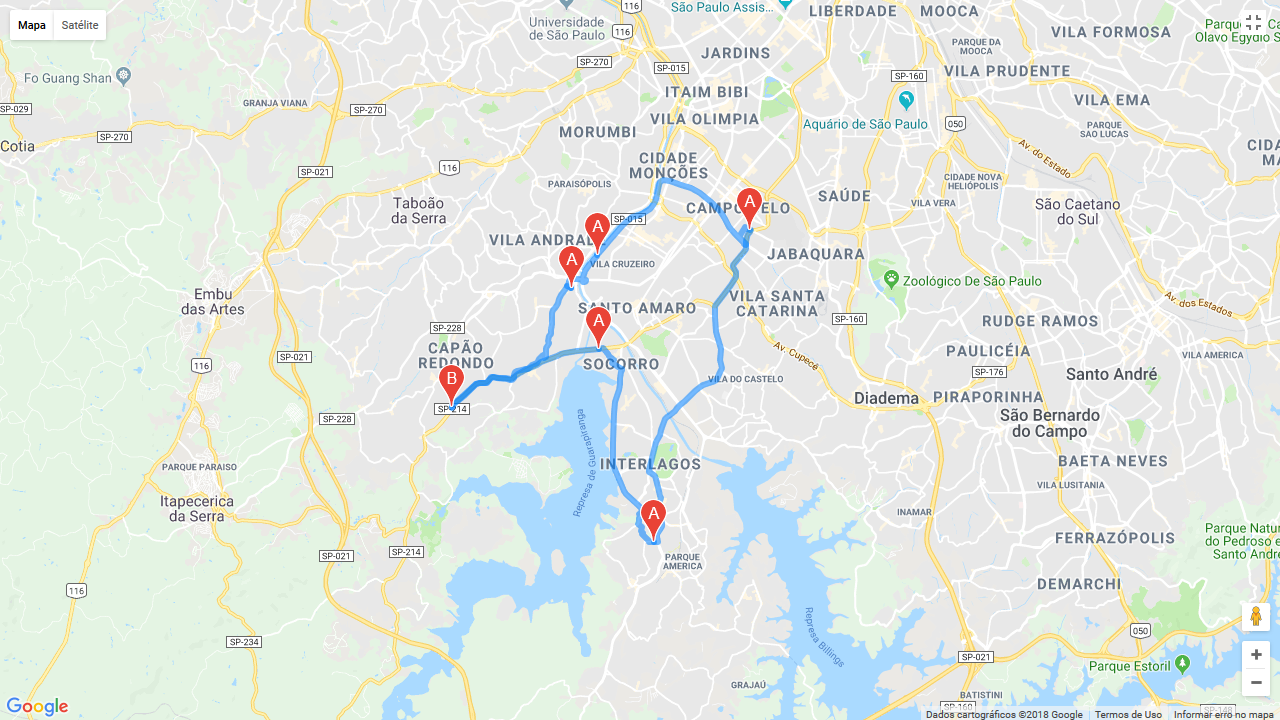
\includegraphics[keepaspectratio=true,scale=0.5]{../../Analise/Roteiro3/Mapa2.png}}
	\captionof{figure}{Mapa de um de tres entregadores}
	\label{fig:Roteiro3-Mapa2}
\end{center}
\begin{center}
	\makebox[\linewidth]{
		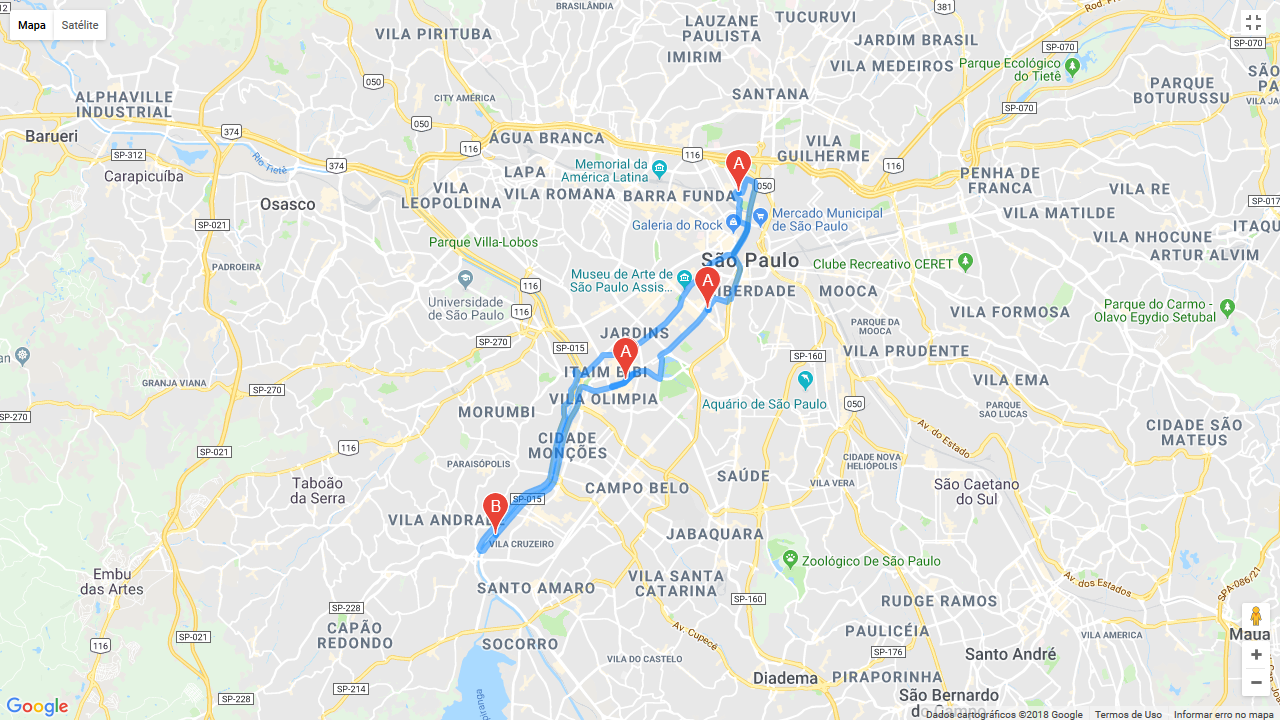
\includegraphics[keepaspectratio=true,scale=0.5]{../../Analise/Roteiro3/Mapa3.png}}
	\captionof{figure}{Mapa de um de tres entregadores}
	\label{fig:Roteiro3-Mapa3}
\end{center}

\subsubsection{500 Gerações e 50 População}
\begin{center}
	\makebox[\linewidth]{
		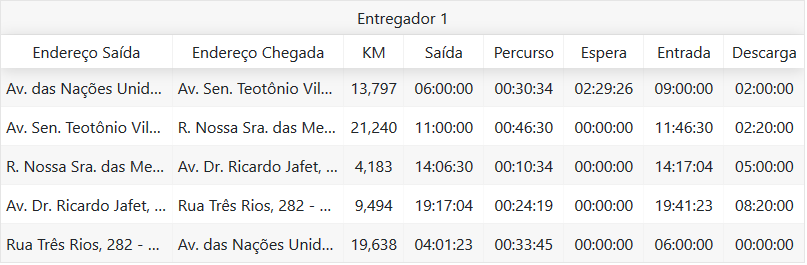
\includegraphics[keepaspectratio=true,scale=0.8]{../../Analise/Roteiro3/G500P50/DisplacementMutation.png}}
	\captionof{figure}{Mutação DisplacementMutation}
	\label{fig:Roteiro3-G500P50-DisplacementMutation}
\end{center}
\begin{center}
	\makebox[\linewidth]{
		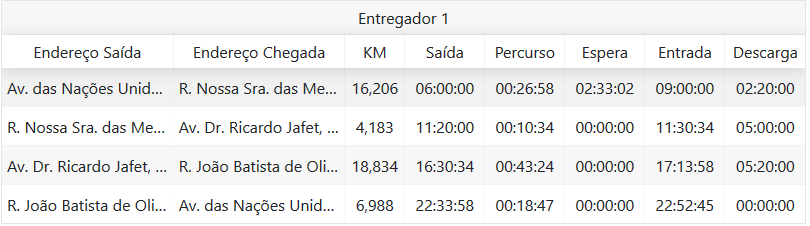
\includegraphics[keepaspectratio=true,scale=0.8]{../../Analise/Roteiro3/G500P50/InsertionMutation.png}}
	\captionof{figure}{Mutação InsertionMutation}
	\label{fig:Roteiro3-G500P50-InsertionMutation}
\end{center}
\begin{center}
	\makebox[\linewidth]{
		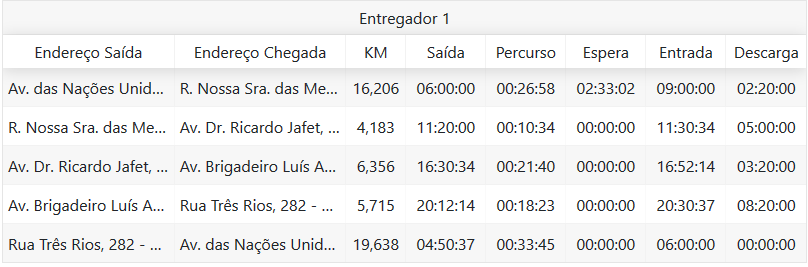
\includegraphics[keepaspectratio=true,scale=0.8]{../../Analise/Roteiro3/G500P50/InversionMutation.png}}
	\captionof{figure}{Mutação InversionMutation}
	\label{fig:Roteiro3-G500P50-InversionMutation}
\end{center}
\begin{center}
	\makebox[\linewidth]{
		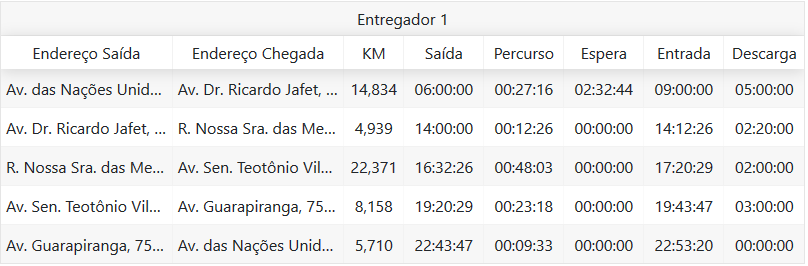
\includegraphics[keepaspectratio=true,scale=0.8]{../../Analise/Roteiro3/G500P50/SwapMutation.png}}
	\captionof{figure}{Mutação SwapMutation}
	\label{fig:Roteiro3-G500P50-SwapMutation}
\end{center}

\subsubsection{1000 Gerações e 100 População}
\begin{center}
	\makebox[\linewidth]{
		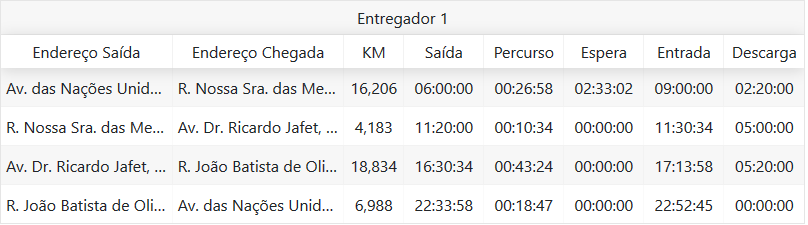
\includegraphics[keepaspectratio=true,scale=0.8]{../../Analise/Roteiro3/G1000P100/DisplacementMutation.png}}
	\captionof{figure}{Mutação DisplacementMutation}
	\label{fig:Roteiro3-G1000P100-DisplacementMutation}
\end{center}
\begin{center}
	\makebox[\linewidth]{
		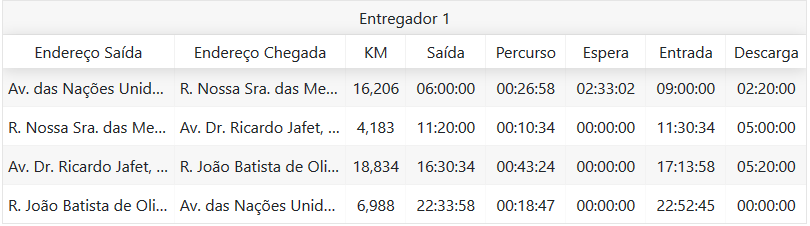
\includegraphics[keepaspectratio=true,scale=0.8]{../../Analise/Roteiro3/G1000P100/InsertionMutation.png}}
	\captionof{figure}{Mutação InsertionMutation}
	\label{fig:Roteiro3-G1000P100-InsertionMutation}
\end{center}
\begin{center}
	\makebox[\linewidth]{
		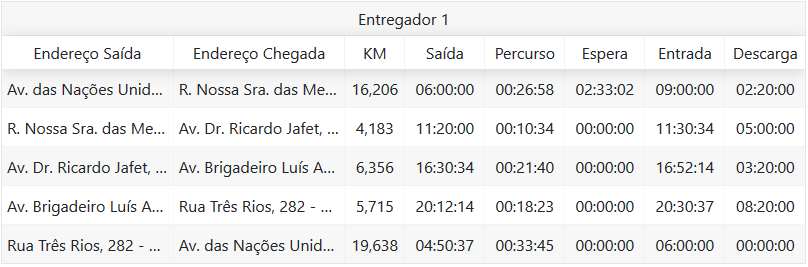
\includegraphics[keepaspectratio=true,scale=0.8]{../../Analise/Roteiro3/G1000P100/InversionMutation.png}}
	\captionof{figure}{Mutação InversionMutation}
	\label{fig:Roteiro3-G1000P100-InversionMutation}
\end{center}
\begin{center}
	\makebox[\linewidth]{
		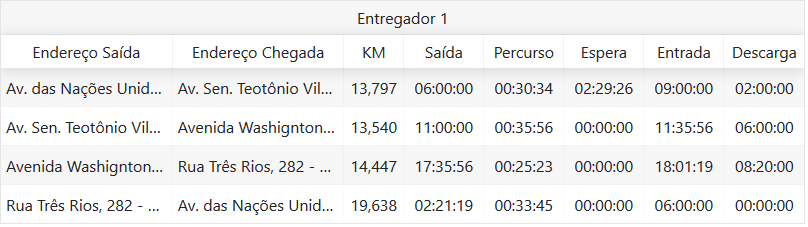
\includegraphics[keepaspectratio=true,scale=0.8]{../../Analise/Roteiro3/G1000P100/SwapMutation.png}}
	\captionof{figure}{Mutação SwapMutation}
	\label{fig:Roteiro3-G1000P100-SwapMutation}
\end{center}



\subsection{Alteração do tempo com base no transito}
\subsubsection{Média}
\begin{center}
	\makebox[\linewidth]{
		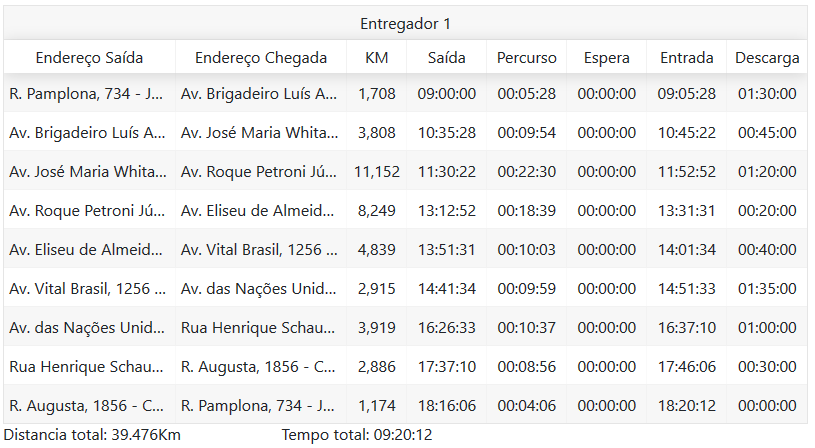
\includegraphics[keepaspectratio=true,scale=0.8]{../../Analise/Situacoes/Media.png}}
	\captionof{figure}{Rota gerada com a média do historico de transito}
	\label{fig:RoteiroMedia}
\end{center}
\subsubsection{Otimista}
\begin{center}
	\makebox[\linewidth]{
		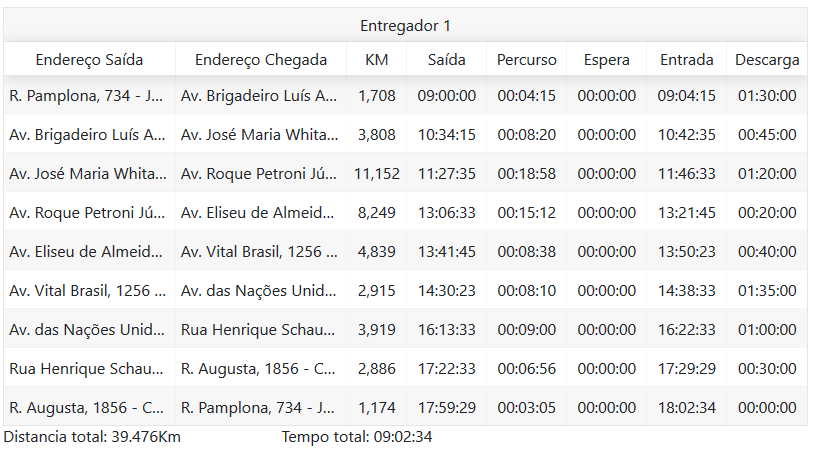
\includegraphics[keepaspectratio=true,scale=0.8]{../../Analise/Situacoes/Otimista.png}}
	\captionof{figure}{Rota gerada com o melhor tempo de cada rota}
	\label{fig:RoteiroOtimista}
\end{center}
\subsubsection{Pessimista}
\begin{center}
	\makebox[\linewidth]{
		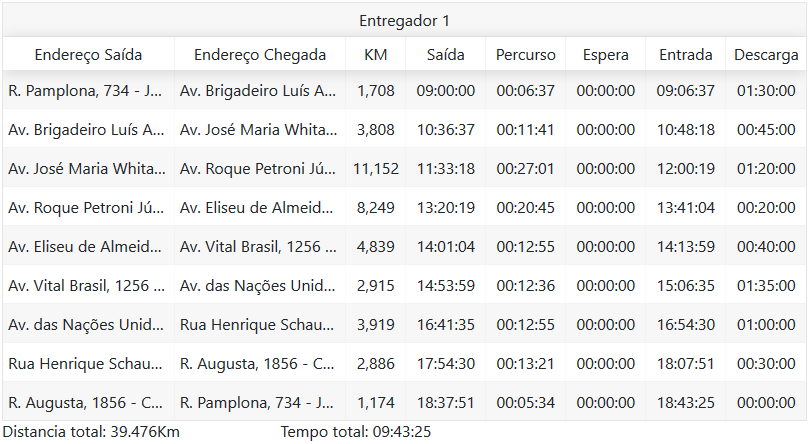
\includegraphics[keepaspectratio=true,scale=0.8]{../../Analise/Situacoes/Pessimista.png}}
	\captionof{figure}{Rota gerada com o pior tempo de cada rota}
	\label{fig:RoteiroPessimista}
\end{center}

\subsection{Roteiro não é possível entregar}
\begin{center}
	\makebox[\linewidth]{
		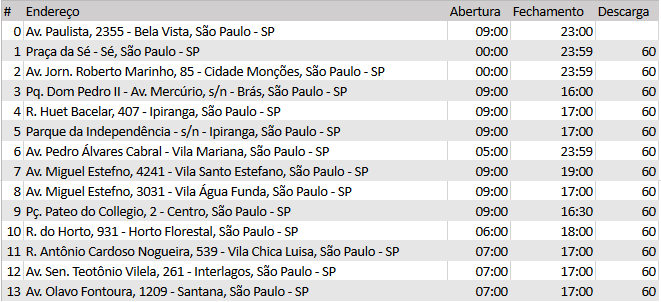
\includegraphics[keepaspectratio=true,scale=1.0]{../../Analise/RoteiroNaoepossivelentregar.png}}
	\captionof{figure}{Roteiro não é possível entregar}
	\label{fig:RoteiroNaoepossivelentregar}
\end{center}




\subsection{Roteiro Não é possível entregar com apenas 1}
\begin{center}
	\makebox[\linewidth]{
		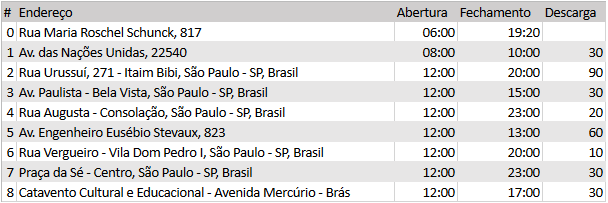
\includegraphics[keepaspectratio=true,scale=1.1]{../../Analise/RoteiroNaoepossivelentregarcomapenas1.png}}
	\captionof{figure}{Roteiro Não é possível entregar com apenas 1}
	\label{fig:RoteiroNaoepossivelentregarcomapenas1}
\end{center}

\section{Conclusão}

Neste trabalho, apresentamos a aplicação de uma abordagem evolutiva genérica para o PRVJT. A solução provou ser extremamente eficaz, uma vez que fomos capazes de encontrar rotas otimizadas para varias combinações de endereço de entrega. Além disso, os resultados mostram que este método é robusto e escalável. 
Fomos capazes de criar uma aplicação Web, com interface simples, para realizar os cálculos em tempo real, o que significa que o sistema consegue encontrar uma solução com uma velocidade relativamente alta, ja que existe um tempo limite \textit{timeout} em requisições HTTP.

O Google Maps ajudou na definição da rota por entregar o transito médio da rota fazendo com que o caminho escolhido pelo software fique mais próximo de uma situação real. 

O GA ajudou na escolhas das rotas para minimizar o tempo, a distância e o numero de entregadores, encontrando padrões difíceis de ser vistos, porém, para encontrar uma solução próxima do ótimo é preciso perder performance para calcular a resposta, aumentando o numero de gerações e população para encontrar a rota.

Utilizando um número baixo de destinos o processo de recalculo de rotas para cada vez que chegar em um  destino, se mostra útil para identificar mudanças no transito e ainda chegar no horário proposto.

\section{Trabalhos futuros}

Devido a média de tempo para se encontrar as rotas, avaliar a possível paralelização da rotina de algoritmos genéticos.

Aplicar mais uma restrição, como uma quantidade máxima de carga por entregador.

Desenvolver um aplicativo mobile para avançar as próximas rotas para cada entregador.

Utilizar uma base de dados maior para os testes, baseada em casos reais de logística.